\documentclass[tikz, border=10pt]{standalone}
\usepackage[utf8]{inputenc}
\usetikzlibrary{shapes.geometric, arrows.meta, positioning, fit, backgrounds, calc}

\begin{document}
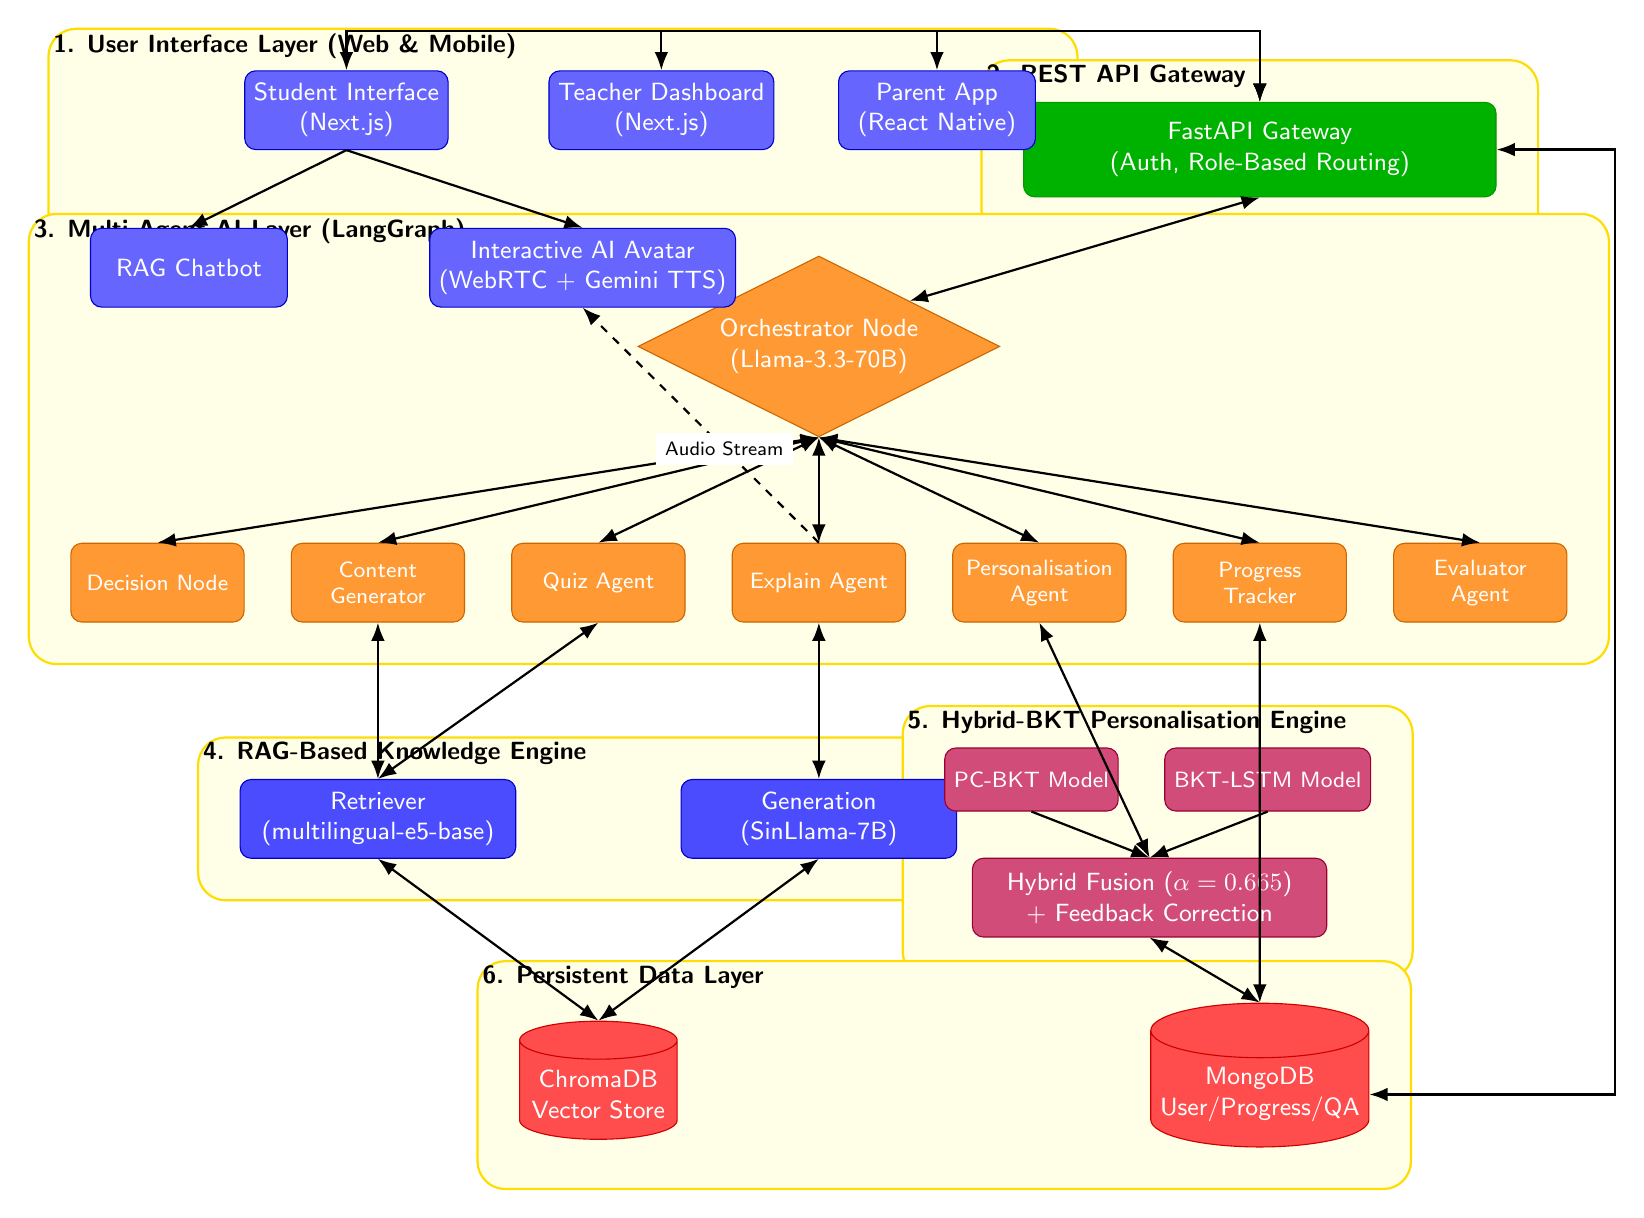
\begin{tikzpicture}[
    % Styles
    ui layer/.style={fill=yellow!10, draw=yellow!80!orange, thick, inner sep=15pt, rounded corners=10pt},
    ui node/.style={rectangle, draw=blue!80!black, fill=blue!60!white, text=white, align=center, font=\small\sffamily, minimum height=1cm, minimum width=2.5cm, rounded corners},
    api node/.style={rectangle, draw=green!60!black, fill=green!70!black, text=white, align=center, font=\small\sffamily, minimum height=1.2cm, minimum width=6cm, rounded corners},
    agent node/.style={rectangle, draw=orange!80!black, fill=orange!80, text=white, align=center, font=\footnotesize\sffamily, minimum height=1cm, minimum width=2.2cm, rounded corners},
    orch node/.style={diamond, draw=orange!80!black, fill=orange!80, text=white, align=center, font=\small\sffamily, aspect=2, minimum width=3cm},
    rag node/.style={rectangle, draw=blue!80!black, fill=blue!70, text=white, align=center, font=\small\sffamily, minimum height=1cm, minimum width=3.5cm, rounded corners},
    bkt node/.style={rectangle, draw=purple!80!black, fill=purple!70, text=white, align=center, font=\footnotesize\sffamily, minimum height=0.8cm, minimum width=2cm, rounded corners},
    bkt fusion/.style={rectangle, draw=purple!80!black, fill=purple!70, text=white, align=center, font=\small\sffamily, minimum height=1cm, minimum width=4.5cm, rounded corners},
    db node/.style={cylinder, shape border rotate=90, draw=red!80!black, fill=red!70, text=white, align=center, font=\small\sffamily, aspect=0.25, minimum height=1.5cm, minimum width=2cm},
    arrow/.style={-Latex, thick},
    dbl arrow/.style={Latex-Latex, thick},
    dashed arrow/.style={-Latex, dashed, thick},
    layer label/.style={font=\small\sffamily\bfseries, anchor=north west, inner sep=2pt}
]

% Center is Orchestrator at (0, 0)
\node[orch node] (orch) at (0,0) {Orchestrator Node\\(Llama-3.3-70B)};

% Layer 3 Agents (Y = -3)
\node[agent node] (explain) at (0, -3) {Explain Agent};
\node[agent node] (quiz) at (-2.8, -3) {Quiz Agent};
\node[agent node] (content) at (-5.6, -3) {Content\\Generator};
\node[agent node] (decision) at (-8.4, -3) {Decision Node};

\node[agent node] (pers) at (2.8, -3) {Personalisation\\Agent};
\node[agent node] (prog) at (5.6, -3) {Progress\\Tracker};
\node[agent node] (eval) at (8.4, -3) {Evaluator\\Agent};

% Layer 2 API Gateway
\node[api node] (api) at (5.6, 2.5) {FastAPI Gateway\\(Auth, Role-Based Routing)};

% Layer 1 UI
\node[ui node] (teacher) at (-2, 3) {Teacher Dashboard\\(Next.js)};
\node[ui node] (student) at (-6, 3) {Student Interface\\(Next.js)};
\node[ui node] (parent) at (1.5, 3) {Parent App\\(React Native)};

\node[ui node] (avatar) at (-3, 1) {Interactive AI Avatar\\(WebRTC + Gemini TTS)};
\node[ui node] (chatbot) at (-8, 1) {RAG Chatbot};

% Layer 4 RAG
\node[rag node] (retriever) at (-5.6, -6) {Retriever\\(multilingual-e5-base)};
\node[rag node] (generation) at (0, -6) {Generation\\(SinLlama-7B)};

% Layer 5 BKT
\node[bkt fusion] (fusion) at (4.2, -7) {Hybrid Fusion ($\alpha = 0.665$)\\+ Feedback Correction};
\node[bkt node] (pcbkt) at (2.7, -5.5) {PC-BKT Model};
\node[bkt node] (bktlstm) at (5.7, -5.5) {BKT-LSTM Model};

% Layer 6 DB
\node[db node] (chroma) at (-2.8, -9.5) {ChromaDB\\Vector Store};
\node[db node] (mongo) at (5.6, -9.5) {MongoDB\\User/Progress/QA};

% Connections
\draw[dbl arrow] (student.north) |- ++(0,0.5) -| (api.north);
\draw[dbl arrow] (teacher.north) |- ++(0,0.5) -| (api.north);
\draw[dbl arrow] (parent.north) |- ++(0,0.5) -| (api.north);

\draw[arrow] (student.south) -- (avatar.north);
\draw[arrow] (student.south) -- (chatbot.north);

\draw[dbl arrow] (api.south) -- (orch.north east);

\draw[dbl arrow] (orch.south) -- (decision.north);
\draw[dbl arrow] (orch.south) -- (content.north);
\draw[dbl arrow] (orch.south) -- (quiz.north);
\draw[dbl arrow] (orch.south) -- (explain.north);
\draw[dbl arrow] (orch.south) -- (pers.north);
\draw[dbl arrow] (orch.south) -- (prog.north);
\draw[dbl arrow] (orch.south) -- (eval.north);

\draw[dbl arrow] (content.south) -- (retriever.north);
\draw[dbl arrow] (quiz.south) -- (retriever.north);
\draw[dbl arrow] (explain.south) -- (generation.north);
\draw[dashed arrow] (explain.north) -- node[fill=white, font=\scriptsize\sffamily, pos=0.4] {Audio Stream} (avatar.south);
\draw[dbl arrow] (pers.south) -- (fusion.north);

\draw[arrow] (pcbkt.south) -- (fusion.north);
\draw[arrow] (bktlstm.south) -- (fusion.north);

\draw[dbl arrow] (retriever.south) -- (chroma.north);
\draw[dbl arrow] (generation.south) -- (chroma.north);
\draw[dbl arrow] (prog.south) -- (mongo.north);
\draw[dbl arrow] (fusion.south) -- (mongo.north);
\draw[dbl arrow] (api.east) -- ++(1.5,0) |- (mongo.east);

% Background Boxes
\begin{scope}[on background layer]
    % Layer 1 Box
    \node[ui layer, fit=(student)(parent)(avatar)(chatbot)] (l1) {};
    \node[layer label] at (l1.north west) {1. User Interface Layer (Web \& Mobile)};
    
    % Layer 2 Box
    \node[ui layer, fit=(api)] (l2) {};
    \node[layer label] at (l2.north west) {2. REST API Gateway};
    
    % Layer 3 Box
    \node[ui layer, fit=(orch)(decision)(eval)] (l3) {};
    \node[layer label] at (l3.north west) {3. Multi-Agent AI Layer (LangGraph)};
    
    % Layer 4 Box
    \node[ui layer, fit=(retriever)(generation)] (l4) {};
    \node[layer label] at (l4.north west) {4. RAG-Based Knowledge Engine};
    
    % Layer 5 Box
    \node[ui layer, fit=(pcbkt)(bktlstm)(fusion)] (l5) {};
    \node[layer label] at (l5.north west) {5. Hybrid-BKT Personalisation Engine};
    
    % Layer 6 Box
    \node[ui layer, fit=(chroma)(mongo)] (l6) {};
    \node[layer label] at (l6.north west) {6. Persistent Data Layer};
\end{scope}

\end{tikzpicture}
\end{document}
